\documentclass[11pt]{article}
\title{Policy-First University AI Access: Conditional Safety Guarantees and the Unresolved Case for Campus Federation}
\date{}
\author{SIGMA AI-assisted research synthesis}
\usepackage[T1]{fontenc}
\usepackage[utf8]{inputenc}
\usepackage[margin=1in]{geometry}
\usepackage{amsmath,amssymb,array,booktabs,longtable,pdflscape}
\usepackage{microtype}
\usepackage[hyphens]{url}
\usepackage{xurl}
\usepackage{titlesec}
\usepackage{tikz}
\usetikzlibrary{fit}
\emergencystretch=2em
\raggedbottom
\linespread{1.07}
\usepackage{xcolor}
\definecolor{blue}{HTML}{24485E}
\titleformat{\section}{\Large\bfseries\sffamily\color{blue}}{\thesection}{0.8em}{}
\titleformat{\subsection}{\large\bfseries\sffamily}{\thesubsection}{0.7em}{}
\setlength{\parskip}{.6em}
\setlength{\parindent}{0pt}
\begin{document}
\maketitle

\begin{abstract}
Can universities pool uneven AI capacity without surrendering data authority or exceeding hard budgets? This paper develops a bounded comparison of campus-local inference, approved frontier APIs, a campus gateway with separately approved external access, and a hypothetical inter-campus federation. Its strongest contribution is a set of conditional design constraints rather than a deployment result. A disconnected admission point cannot distinguish unchanged approval from an unseen revocation, while a check followed by an independent send permits a revocation race. A proposed campus-controlled broker narrows authorization to new operating-system transport submissions.

A reservation ledger can preserve spending caps only with complete mediation, enforceable liability bounds, and retained holds for uncertain charges. These mechanisms remain unimplemented and unverified. Actual task quality, capacity, prices, administrative effort, and federation benefit are unknown. A proposed 90-day paired evaluation therefore treats useful completion, policy compliance, financial safety, and incremental federation benefit as separate decision requirements.
\end{abstract}
\section{Introduction and problem statement}
The question is whether federation adds policy-permitted, useful research service beyond a campus gateway with separately approved external access. The comparison defines four alternatives: campus-local inference only, approved frontier API only, a campus gateway with separately approved external access, and a proposed federation extension. Federation and frontier routing are hypotheses about additional architecture, not established MindRouter capabilities.

The unit of service is one offered research task episode, including every descendant model call, tool invocation, retry, and terminal outcome. A useful completion must satisfy authorization, a prespecified task-quality rubric, a latency target, and provenance requirements; refusal and exhaustion remain visible in offered demand. Classroom coding, routine analysis, scientific reasoning, multimodal or long-context work, agent workflows, sensitive tasks, and reproducible batches require separate workload strata rather than a single undifferentiated success score.

Data authority and spending limits are admission constraints, not preferences that a higher model score may override. The proposed comparison retains campus authority over identity, classification, approved destinations, retention, audit, contracts, and quotas, including derived prompts, outputs, logs, embeddings, and caches. The bounded contribution is to identify conditional safety requirements and a falsifiable evaluation design; it does not establish that federation is economical, reliable, or necessary.

\section{Methods and evidence}
The analysis organized the saved evidence around four service alternatives, a root-task unit of analysis, and a common distinction between supplied gateway descriptions and proposed extensions. The starting publications were not retrieved in the saved investigation, so their feature descriptions were treated as project-reported claims rather than inspected publication evidence or measured behavior. The supplied historical review date was not converted into a new access date.

The technical analysis examined indistinguishable policy histories, authorization\textendash{}\allowbreak{}revocation\textendash{}\allowbreak{}submission event orders, and a conditional reservation invariant. It distinguished authorization decisions, durable policy commitment, operating-system transport acceptance, later physical transmission, and recipient receipt. The resulting arguments were assessed as reference-model deductions or proof candidates, not implementation verification.

The comparative analysis separated hypothetical workload arithmetic from observations and examined the saved pilot design and its economic critique. It preserved the offered-demand denominator, independence requirements, multiplicity allocation, and distinction between safety-stop, no-go, and inconclusive outcomes. It also retained the refutation of substituting upper liability estimates for both services' actual costs; no benchmark, fault-injection study, source retrieval, pricing survey, or live pilot was performed.

This synthesis uses a bounded selection of the archived research. Unreviewed records could affect its conclusions; the full omission ledger remains available with the generation record.
\section{The comparison contract}
The comparison asks whether inter-campus federation would add useful, policy-permitted service beyond a campus gateway with separately approved external access, rather than whether it would merely expose more destinations. We define four alternatives with distinct service boundaries: campus-local inference only; approved frontier application programming interfaces (APIs) only; a campus gateway with separately approved external access; and a hypothetical cooperative federation that adds access to eligible capacity at participating campuses. The third alternative is the principal comparator for federation because it already allows local service and independently authorized external use.

Federation must therefore demonstrate an incremental contribution, not claim credit for capabilities available without inter-campus pooling.

MindRouter supplies the published campus-gateway reference for this comparison. Its documentation and PEARC\textquoteright{}26 short paper, identified as starting references reviewed on October 31, 2026, describe protocol translation across OpenAI, Ollama, and Anthropic clients and Ollama and vLLM backends, weighted deficit round-robin fair-share scheduling, per-user quotas, audit logging, and GPU telemetry. These are published capability descriptions, not independently measured performance results in this comparison. The documented service is on campus; neither cooperative federation nor frontier routing is treated here as an existing MindRouter feature.

In particular, the gateway baseline\textquoteright{}s separately approved external access need not imply automatic routing from the gateway to an external provider.

The alternatives differ qualitatively in what they would make available and what would require authorization. Local-only service confines execution to campus capacity but cannot count a task as served merely because some local model accepts it. API-only service considers approved provider destinations, while retaining policy-denied tasks in the demand against which service is assessed. The gateway alternative preserves local service alongside separately approved external access without requiring inter-campus pooling. Federation adds another possible execution domain, but another campus is not presumed eligible simply because it participates in the cooperative arrangement.

For this comparison, each campus retains authority over identity, classification, destinations, retention, audit requirements, contracts, and quotas; uncertain authorization makes a destination ineligible rather than a fallback opportunity.

The unit of analysis is a root-task episode: one user-level research or teaching objective together with the model calls, tool interactions, retries, and continuations undertaken to complete it. A multi-call workflow is therefore one episode, not a collection of independent successful requests. The offered-demand denominator comprises all submitted root-task episodes in the defined workload, including those refused, left queued, or otherwise unfinished. This prevents an alternative from appearing more reliable merely by excluding work it cannot admit.

Each alternative is to be assessed over the same prespecified execution horizon, with common rules for submission cutoffs and unfinished episodes; requests still unresolved at the cutoff remain visible rather than disappearing from the comparison.

We propose seven workload reporting strata: classroom coding, routine analysis, demanding scientific reasoning, multimodal or long-context work, agentic multi-call workflows, sensitive-data tasks, and reproducible batches. These labels define comparison categories, not an observed workload distribution or evidence that any alternative can support them. Because sensitivity and reproducibility can overlap the other categories, stratum membership need not be exclusive, but each root-task episode enters the aggregate denominator only once.

The workload specification must establish the requested result, applicable data restrictions, deadline, and required provenance before execution, so that easy acceptance or rapid response cannot substitute for task completion.

The primary outcome is joint success at the episode level: execution must remain authorized, the result must meet the task\textquoteright{}s quality criterion, completion must occur within its deadline, and the required provenance must be available. These conditions are conjunctive; a high-quality answer reached through an unauthorized destination is not a successful episode, and an authorized response that fails the task is not useful completion. Provenance requirements should identify the model or version and execution information needed for the particular task, without assuming that every task requires identical reproducibility.

Task-qualified evaluators must be appointed to establish and apply the quality criteria, while campus-designated security and data-policy evaluators must assess authorization and handling requirements. These are necessary evaluation roles, not assessments already performed.

Latency, throughput, availability, provenance completeness, and administrative burden remain distinct comparison outcomes rather than substitutes for joint success. Budget compliance likewise remains a separate requirement: a useful result does not establish that its execution respected a hard spending limit. No measured ranking of the four alternatives follows from the supplied gateway descriptions. The comparison contract instead makes the federation claim narrower and testable: its value must come from additional authorized, adequate, timely, and sufficiently documented root-task completions relative to the gateway baseline under comparable demand and budget constraints, not from destination count or successful individual calls.

\section{Policy-first routing and revocation limits}
Policy-first routing makes campus permission a prerequisite for optimization, rather than a factor that quality, speed or cost can outweigh. The proposed rule first determines which destinations may receive a request and its associated data; only within that eligible set may the router compare task-specific quality, latency, reproducibility and incremental cost. The central constraint is temporal: permission at submission does not necessarily authorize a later release. Two counterexamples establish why cached approval and an independent check-before-send operation are insufficient under a strict revocation contract.

Eligibility begins with authentication, project attribution and resolution of effective data restrictions. A candidate destination must satisfy home-campus approval, destination acceptance, retention, audit and contractual conditions, model and GPU-memory fit, and available authorized budget. Ambiguous classification excludes off-domain candidates. Overload, provider rejection, exhausted quota or a better estimated answer cannot enlarge this set; when no destination qualifies, the permitted responses are authorized local queuing or a visible refusal, not an unapproved fallback.

The proposed classification discipline applies to derived objects as well as original inputs. Let $L(x)$ denote the restrictions attached to an object $x$; for an object $y$ derived from inputs $x_i$, require $L(y) \supseteq \bigcup_i L(x_i)$ unless authorized declassification explicitly changes those restrictions. Outputs, tool results, embeddings, caches and diagnostic records therefore do not become less restricted merely through transformation. This is a conservative information-flow specification, not evidence that an automatic classifier can reliably identify sensitive content from text alone.

For the revocation analysis, an egress event is the release of a data-bearing unit through a managed boundary, including request bodies, streamed output, tool arguments, logs, cache writes and content-bearing telemetry. The proposed immediate-revocation contract requires a revocation ordered before such an event by the home-campus authority to govern that event. It does not require recall of previously released data, and it is an analytical premise rather than an established campus policy. The unit of analysis is a single controlled release; the counterexample horizon contains only one request following one possible revocation, and the outcome criterion is whether dispatch satisfies that ordering requirement.

Consider a gateway $G$ with cached permission for project $J$ to send data of class $D$ to partner $B$. After caching that permission, $G$ loses communication with the home authority $A$ but retains connectivity to the requester and $B$. In history $H_0$, the authority leaves permission unchanged; in history $H_1$, it revokes permission before the next request arrives. Give the gateway identical requests, clock readings and network observations in both histories, with no revocation message able to cross the partition. Its local state at the dispatch decision is then identical despite the different authoritative policies.

A deterministic gateway must make the same decision in both histories, while a randomized gateway must use the same decision distribution. Let $p$ be its dispatch probability under those identical observations: dispatch availability in $H_0$ and unauthorized-dispatch probability in $H_1$ are both $p$. Requiring availability of at least $a$ and violation probability of at most $\varepsilon$ therefore requires $a \leq p \leq \varepsilon$, and hence $a \leq \varepsilon$. Guaranteed dispatch and zero violations cannot coexist under these premises; denying or waiting preserves this authorization condition at the expense of partition-time dispatch availability.

This is a logical counterexample, not an observed benchmark, incident frequency or reliability estimate.

Cached signatures, policy-version fields and allocation mechanisms do not supply the missing information. A signature establishes who issued an approval, not whether it has subsequently been revoked; a version field cannot reveal an unseen newer version, and fair-share scheduling or quotas cannot establish destination authorization. A lease can instead define permission as valid until expiry despite an intervening revocation, with exposure bounded by the remaining lease duration only under trusted clocks and explicitly accepted lease semantics. That changes the contract rather than satisfying immediate revocation.

The counterexample therefore concerns a particular combination of guarantees, not federation generally: remote dispatch can remain permissible when the home authority is reachable or when the campus explicitly adopts a different revocation contract.

Even without a partition, a separate policy check followed by transmission admits a second counterexample. The schedule \[\operatorname{check}(v_0) \prec \operatorname{revoke}(v_1) \prec \operatorname{release}(v_0)\] permits release using an approval that was valid when checked but revoked before release. Moving the check closer to transmission does not exclude this ordering; nor does reusing authorization from an earlier job admission. Every retry, agent subcall and tool call consequently requires fresh admission, and the selected destination must still pass a release-time gate. Queued work and streaming make the distinction consequential because authorization of a job is not authorization of every later data-bearing event.

A narrower conditional guarantee is available if trusted classification, authenticated destinations, complete mediation and serialization of policy changes with controlled releases are assumed. Define the authorization invariant to require, at each release, an authenticated campus principal, current permission for the object's restrictions, the required destination and retention agreement, and any necessary budget reservation. Starting from an empty release history, rejection adds no event, while acceptance adds only an event satisfying those predicates; induction then preserves the invariant over every finite controlled-egress history.

The check\textendash{}\allowbreak{}revoke\textendash{}\allowbreak{}send schedule violates the serialization premise rather than refuting this conditional argument. A component inventory alone does not establish that premise, particularly for queued work, streaming and crash recovery.

The resulting design obligation is to specify the revocation contract and its controlled release boundary before claiming that additional destinations improve policy-compliant availability. Authorization at that boundary does not establish recipient retention, deletion or incident-response compliance, which require separate contractual and technical evidence. For the federation comparison, cached approval is therefore insufficient evidence of usable partner capacity: capacity counts only when the destination is eligible and the release can meet the campus's chosen revocation semantics.

The negative result rules out an unconditional combination of immediate revocation and disconnected dispatch, while leaving open whether federation provides incremental authorized service under an explicit, enforceable contract.

\section{The proposed controlled release boundary}
A campus-controlled broker could close the authorization race by making committed policy updates and new operating-system transport submissions share one serialization boundary. The proposal places authority over managed releases and ownership of their outbound sockets in the same campus-controlled component, rather than treating an earlier policy check as permission to send later. This is a specification proposal: no implementation or executed fault-injection study establishes its mediation, transport, recovery, or ownership premises, and the supplied evidence does not establish these mechanisms as MindRouter capabilities.

The analytical workload consists of bounded, immutable content units submitted across a managed boundary, including successive chunks of a stream. The unit of analysis is a positive-length prefix accepted by the operating-system transport, and the authorization result concerns every finite event history satisfying the specified transitions, not an observed service period. Its outcome oracle asks whether each acceptance was permitted by the last preceding committed policy in the broker\textquoteright{}s serialization order. Campus security must decide whether that boundary meets institutional requirements; independent implementation testing remains necessary to establish that an actual system realizes it.

Let $B$ denote the broker and $M$ its exclusive serialization gate. An authenticated administrative update becomes effective only when $B$ durably commits it under $M$; an administrator issuing the request, the broker receiving it, and an intent record being written are not themselves policy commitment. Acknowledgment follows the durable commit. Release is defined separately as acceptance of a positive byte count by the outbound operating-system transport during a synchronous, nonblocking submission operation\textemdash{}not application enqueueing, physical packet transmission, or recipient receipt. [[Research session 2, artifact 5]]

Complete mediation is an essential premise of this boundary. In the proposed design, only the broker holds destination credentials and owns managed outbound connections; workers and tenants have no alternative managed egress. Each content unit binds its bytes, classification, authenticated principal and project, destination and connection identity, retention and contract requirements, and reservation identifier; changing a binding requires revalidation. Streaming, tool calls, logs, embeddings, caches, and content-bearing telemetry require equivalent treatment wherever they cross an approved boundary.

Trusted classification and broker and operating-system enforcement are assumed: tenant manipulation of a label cannot confer authority, while compromise of those trusted components falls outside the conditional guarantee.

The broker starts disabled during recovery. A final submission may proceed only while recovery is complete, exclusive ownership is enforceably valid, classification is unambiguous, the immutable binding is permitted by committed policy, cancellation and destination requirements pass, and sufficient durable reservation coverage remains. Under $M$, the broker performs this final validation, durably records an ARMED intent, immediately makes one nonblocking transport submission, and classifies its result before releasing the gate. Policy commitment uses the same gate, so it cannot intervene between validation and acceptance.

ARMED is therefore a write-ahead record, not an independently executable permission; a detached outbox worker would not satisfy this rule.

The authorization argument follows directly from that shared ordering. Initially there are no releases; for each subsequent positive acceptance, complete mediation places the operation inside the final submission path, and the gate preserves the validated policy through the operating-system call. Immutable bindings prevent substitution of different content or a different destination, while effective ownership enforcement excludes an unauthorized broker. Rejected operations and certified zero-acceptance calls add no release, yielding the invariant by induction over finite histories.

If a call accepts only a prefix of length $n>0$, only that prefix is released; the remainder and every subsequent streaming chunk require a new final validation. [[Research session 2, artifact 6]]

This invariant does not establish a physical cutoff at revocation. A transport acceptance can precede a committed revocation while the corresponding packet transmission or recipient receipt follows it; previously accepted bytes may remain buffered or be retransmitted. Conversely, an application or TLS queue that independently flushes content after the broker\textquoteright{}s validation would break the proposed operating-system boundary, because its eventual socket submission would escape the shared gate. Encryption may prepare immutable bytes inside the trusted broker, but actual socket submissions must still pass through the controlled path.

The contract neither recalls prior submissions nor establishes downstream deletion, cessation of processing, or recipient compliance.

Administrative connectivity must also be distinguished from broker authority. If an administrator creates a revocation but the request never reaches an otherwise functioning, exclusively authorized broker, the last committed policy remains effective and may still permit submission. The same holds for a received but uncommitted update: this specification supplies no separate pending-update barrier. Once revocation commits, later submissions\textemdash{}including unsent suffixes and new streaming chunks\textemdash{}must use the updated policy.

Thus the broader generalization that loss of an administrative path necessarily stops release must be withdrawn; the contract provides commit-time revocation, not request-time revocation or a bounded administrative response time, and campus acceptance of that distinction remains outstanding.

A proposed update-status interface would make this distinction observable without confusing delivery with commitment. Each update would have a stable identifier, and a commit receipt would authenticate that identifier, the policy version or digest, the ownership epoch, and the durable commit position. If the receipt is lost, an authoritative, linearizable status query could still establish commitment; a negative answer through a query barrier would establish only that the update had not committed by that barrier.

If the authority cannot be queried, status remains unknown: an administrative timeout, client send success, packet capture, or wall-clock timestamp alone cannot determine whether revocation became effective. [[Research session 2, artifact 6]]

Crash recovery exposes a different uncertainty because a durable intent cannot atomically establish the outcome of a network operation. A crash immediately before transport submission and a crash immediately after acceptance but before durable result logging can leave the same ARMED record. Recovery therefore cannot infer non-dispatch or automatically replay the intent. The proposed recovery procedure keeps submission disabled, establishes termination or fencing of the former owner, restores committed policy and unresolved reservations without rollback, advances the ownership epoch, and marks unfinished attempts uncertain while retaining their reservations.

It closes rather than resumes the affected connections; any later attempt requires fresh validation and coverage for additional liability. [[Research session 2, artifact 5]]

Exclusive ownership requires more than a cached flag or a failure notification. Observed ownership uncertainty disables new transport entry, but an old broker could retain a working socket and submit under stale policy if another authority activates a replacement without fencing it. A sufficient ownership mechanism must order withdrawal against transport admission: either an already admitted operation precedes withdrawal, or withdrawal wins and the operation is rejected. Replacement ownership cannot rely on the former broker being stopped until that fact is enforced across every managed submission path, including in-flight calls.

Without such enforcement, the specification supports rejection after observed disablement, not after an invisible ownership loss.

The decisive implementation evidence would correlate immutable content-unit identifiers, policy commit positions, gate-operation order, and ownership decisions with independently collected kernel socket-acceptance events and returned byte counts. Each positive acceptance would then be checked against the preceding committed policy and valid ownership epoch; an SDK enqueue or a packet arriving after revocation would not substitute for that observation. Missing traces or a crash between acceptance and durable result logging would remain unknown rather than count as successful enforcement.

The resulting argument is narrower but more actionable: campus control can be specified at new transport submission, whereas request delivery, buffered transmission, recipient behavior, and ownership handoff require distinct assurances that a routing decision alone cannot supply. [[Research session 2, artifact 6]]

\begin{figure}[!htbp]
\centering
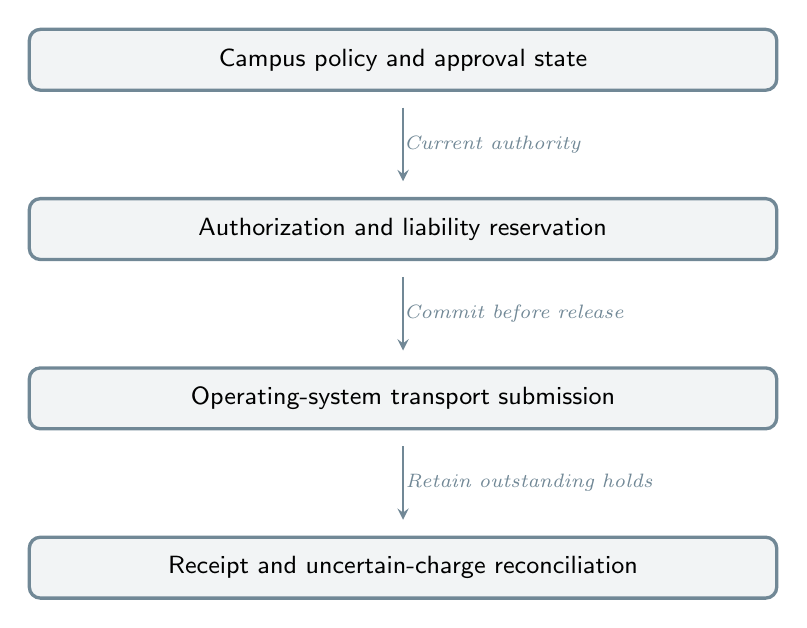
\begin{tikzpicture}[x=1cm,y=1cm,>=stealth,story node/.style={draw=blue!65,very thick,rounded corners=4pt,align=center,text width=9cm,font=\small\sffamily,fill=blue!6,inner sep=7pt}]
\node[story node] (policy) at (0,0.00) {Campus policy and approval state};
\node[story node] (admission) at (0,-2.15) {Authorization and liability reservation};
\node[story node] (send) at (0,-4.30) {Operating-system transport submission};
\node[story node] (reconcile) at (0,-6.45) {Receipt and uncertain-charge reconciliation};
\draw[->,thick,blue!65,shorten <=2mm,shorten >=2mm] (policy) -- node[midway,right,font=\scriptsize\itshape,align=left,text width=3.8cm,fill=white,inner sep=1pt] {Current authority} (admission);
\draw[->,thick,blue!65,shorten <=2mm,shorten >=2mm] (admission) -- node[midway,right,font=\scriptsize\itshape,align=left,text width=3.8cm,fill=white,inner sep=1pt] {Commit before release} (send);
\draw[->,thick,blue!65,shorten <=2mm,shorten >=2mm] (send) -- node[midway,right,font=\scriptsize\itshape,align=left,text width=3.8cm,fill=white,inner sep=1pt] {Retain outstanding holds} (reconcile);
\end{tikzpicture}
\caption{Proposed campus-controlled release path. Authorization and budget reservation must precede the operating-system send boundary; later receipt and charge reconciliation do not retroactively authorize a forbidden submission. This is a conditional design, not a deployed system.}
\par\smallskip{\scriptsize Source-linked claims: C10, C11, C12; evidence links appear in the claim notes.}
\end{figure}
\section{Hard budgets under uncertain billing}
Hard-budget protection requires reserving possible liability before dispatch, rather than treating a missing response as evidence that no expense occurred. The proposed accounting rule separates financial safety from useful availability: retaining an uncertain charge can preserve a cap while preventing a retry that would otherwise complete useful work. Its contribution is a conditional invariant for gateway-controlled spending, not an observed reliability result or an established MindRouter capability. [C10\textendash{}\allowbreak{}C11]

The accounting workload comprises every potentially billable attempt mediated by the gateway, including tool calls, agent continuations and independently chargeable retries. The unit of analysis is an attempt\textquoteright{}s liability to each applicable budget account during a billing window; the analytical horizon covers any sequence of permitted ledger transitions, including unresolved charges carried across window boundaries. Final contractual settlement, a binding determination of no charge, or verified billing deduplication supplies the financial outcome oracle; a timeout alone does not. These definitions support an accounting argument without implying measured task completion or service reliability. [C10\textendash{}\allowbreak{}C11]

For account $k$, let $B_k$ denote its cap, $F_k$ finalized spending and $H_k$ the total outstanding reservations. An attempt $a$ requires an enforceable upper liability bound $r_{ak}$ covering its entire possible charge to that account, including applicable tokens, tools, service-internal retries, fees and currency exposure. A bounded output length is insufficient if other chargeable activity remains unbounded; such an attempt must be rejected or placed under an enforceable contractual bound. Fixed commitments must already appear in finalized spending or reservations, while partially billed but unresolved attempts remain wholly represented by their holds rather than also being counted in finalized spending.

User, project, department and campus limits overlap intentionally. The same expense consumes an equal amount of each applicable limit, but those account balances are not summed to calculate campus expenditure: the campus ledger records the expense once. Admission must reserve against all applicable accounts atomically, so concurrent requests cannot each rely on capacity that another request has already committed. For multi-call workflows, either each potentially billable continuation re-enters admission or a bounded parent envelope allocates child reservations without reusing the same reserved capacity.

The initial condition is $F_k+H_k\leq B_k$ for every account. Admission of attempt $a$ is permitted only if $F_k+H_k+r_{ak}\leq B_k$ holds for every applicable account, after which the ledger atomically adds the reservation. Dispatch itself does not change accounted liability. At final settlement, replacing the reservation with actual charge $c_{ak}$, where $0\leq c_{ak}\leq r_{ak}$, changes the total by $c_{ak}-r_{ak}\leq0$. Induction over these serialized transitions therefore preserves each cap under the stated accounting contract.

A hold may be released for a certified never-sent attempt without adding a charge, but an unknown outcome, timeout or cancellation request leaves it unchanged. A potentially chargeable retransmission requires another reservation unless verified provider deduplication covers the charges; crash recovery must not treat uncertainty about the first transmission as permission to spend its reservation again. Unresolved liability also cannot disappear when a billing window resets: it requires a cross-window encumbrance or an explicitly bounded contractual assignment to a window. These rules preserve the distinction between released capacity and merely unobserved spending. [C10\textendash{}\allowbreak{}C11]

The financial assumptions are consequential: complete mediation of spending, a durable authoritative ledger with atomic multi-account updates, enforceable liability bounds and settlement no greater than the reserved amount. Unauthorized credentials and independent purchases fall outside this guarantee. Dated contractual terms governing maximum charges, cancellation, timeout settlement and billing deduplication remain necessary, as does independent fault testing of concurrency, crashes, duplicate transmissions and billing-window transitions. Neither those provider properties nor implementation correctness has been established by the analytical derivation.

The constructed timeout example isolates why uncertainty cannot safely be converted into available budget. Let the remaining budget be $b>0$, and let each attempted call cost exactly $b$; after the first request, the campus observes a timeout in either of the two histories shown in the table. Releasing the first reservation and issuing an independently billable retry can create liability of $2b$ against available budget $b$, whereas retaining it can block useful work even when the first request incurred no charge. This is a counterexample to timeout-based release, not an observed provider incident or a counterexample to federation itself.

Distinguishing those histories requires information that the timeout does not provide. A binding no-charge receipt, final billing reconciliation, or documented and tested idempotency covering billing and all tool effects could change the retry decision. A cancellation acknowledgement is insufficient unless its contract establishes final liability. Without such information, strict spending safety and an unconditional immediate retry cannot both be guaranteed when the first attempt may have consumed the remaining budget.

Zero-budget operation is the limiting case of the same admission rule. With no prior funding, $B_k=0$ and nonnegative finalized spending and reservations, no new attempt with $r_{ak}>0$ can pass admission. Exhaustion must therefore produce denial or an independently authorized alternative that does not draw on the exhausted paid budget, rather than paid retry escalation; this does not imply that campus-local inference has no incremental or fully loaded cost. The accounting result thus makes retained liability a constraint on the central access argument: additional destinations, including a hypothetical federation, do not remove the need to fund each possible charge or resolve uncertainty before reusing its hold. [C10\textendash{}\allowbreak{}C12]

\section{Costs and bounded scenario arithmetic}
The economic comparison turns on the cost of useful, policy-permitted research work, not on nominal GPU capacity or advertised token prices. Campus-local inference, approved API access, a campus gateway with separately approved external access, and a hypothetical federation must therefore be compared over the same offered workload and accounting horizon. Separate cost bases are necessary because the least expensive use of already-owned equipment need not be the least expensive long-term service, and neither establishes whether federation adds sufficient useful service to justify its overhead.

For the bounded arithmetic below, the workload is a hypothetical monthly cohort, and the unit of analysis is a root-task episode rather than an individual model call. A useful completion must jointly satisfy authorization, task-specific quality, deadline, and provenance requirements; calls, tools, and retries are descendants of that episode, not additional completed tasks. Applying this outcome rule requires appointed task-quality and security evaluators, while campus computing and procurement must substantiate resource and charging inputs; the supplied evidence contains no completed assessments by these roles.

The local-capacity ledger should distinguish sunk expenditure, incremental expenditure attributable to the compared service, and fully loaded ownership and operating cost. GPU acquisition and replacement payments belong in a dated cash-flow schedule, whereas depreciation belongs in the ownership-cost account; adding both as expenses for the same asset and period would double-count its capital contribution. Similarly, an incremental comparison should include only demonstrably additional or avoidable costs, rather than assuming that existing staff, equipment, or support expenditure disappears when work moves elsewhere.

Local inputs include GPU purchase and replacement timing, utilization and idle capacity, power, cooling, storage, network, hardware support, procurement, and staff operations. Utilization must be associated with the workload that the hardware can actually serve, so idle or incompatible capacity cannot be credited as completed research work. Staff scope and shared-resource allocations require a non-overlapping ledger, and sensitivity to utilization and demand must not assume that usefulness remains constant through saturation.

The API ledger should record provider, model or service version, effective price date, billing unit, and separate input, output, and cached-input rates. It must include the complete workflow: repeated reasoning or agent calls, retries, tools, embeddings, egress, and minimum commitments, with contractual liabilities reconciled against usage charges rather than indiscriminately added to them. Cache-dependent savings and ambiguous timeout or cancellation charges require explicit treatment, because an expected cache hit or an unsuccessful response does not establish the maximum financial exposure.

Current dated prices, charging terms, campus ledgers, and federation overhead have not been established, so monthly and annual monetary totals remain unfilled rather than being populated from uninspected illustrative figures.

For each baseline and explicitly named cost basis, reporting should include total cost, cost per active researcher, and cost per useful completed episode over the same horizon. If $C_b$ is the cost of baseline $b$, $R_b$ its active-researcher count, and $S_b$ its observed useful-completion count, the latter measures are $C_b/R_b$ and $C_b/S_b$ when their denominators are positive; a scenario ratio using expected completions must be labelled as such. Annual accounting also requires the applicable acquisition, replacement, operating, and contractual schedules, not an unsupported extrapolation from a single illustrative month.

Across the gateway and federation alternatives, shared costs must be counted once and genuinely additional coordination or administrative costs identified separately.

The hypothetical cohort contains $2{,}000$ monthly root tasks: $200$ sensitive campus-only tasks and $1{,}800$ API-eligible tasks. Both campus-local service and the gateway plan admit $200$ sensitive and $800$ other tasks locally, leaving the gateway with $1{,}000$ distinct API-eligible tasks that could receive separately approved external service. These admission counts assume sufficient deadline-feasible capacity; they are not measured campus throughput. Under the additional assumption that each admitted local stratum has average joint usefulness $0.80$, expected local completions are $200\times0.80=160$ sensitive tasks and $1{,}000\times0.80=800$ tasks overall.

The stratum-specific premise is essential and replaces an invalid inference from aggregate usefulness. An overall result of $800$ useful completions among $1{,}000$ local admissions is compatible with zero useful sensitive completions and $800$ useful non-sensitive completions; admitting sensitive tasks first does not repair that inference. Even the repaired expectation of $160$ sensitive completions is not a realized-service guarantee: if all sensitive tasks succeed together with probability $0.80$ and fail together otherwise, the same marginal probabilities produce zero sensitive completions with probability $0.20$.

Independence is unnecessary for summing expectations, but expectations alone do not establish coverage or a predictive guarantee.

A conservative budget illustration can be stated without substituting a token price for a complete episode cost. Let $B$ be the available API budget and $r>0$ a common, enforceable maximum liability per admitted API root; assume complete financial mediation, no opening liabilities or commitments, nonbinding subsidiary quotas, adequate API capacity, and no reuse of reservation savings. The admitted API cohorts are then bounded by $m_G(B)=\min\{1{,}000,\lfloor B/r\rfloor\}$ for the gateway and $m_A(B)=\min\{1{,}800,\lfloor B/r\rfloor\}$ for API-only access.

The table additionally assumes average joint usefulness $0.90$ for every selected API cohort, including budget-truncated cohorts; a full-cohort average would not by itself justify that assumption.

For illustration, the proposed monthly gates are $160$ useful sensitive completions and $1{,}400$ useful completions overall; these are scenario targets, not established university policy. The gateway's expected overall gate requires at least $\lceil(1{,}400-800)/0.90\rceil=667$ API admissions, in addition to the separate sensitive-stratum premise. At API budgets of USD $2{,}000$, USD $4{,}000$, and USD $8{,}000$, this is equivalent to maximum per-root liabilities no greater than approximately USD $2.9985$, USD $5.9970$, and USD $11.9940$, respectively. These are reservation thresholds, not observed average task costs or current API prices; with $B=0$, no paid API roots enter this plan, while local operation still requires funded resources.

The arithmetic describes feasibility only for the declared admission plans and usefulness assumptions. If workload selection, model fit, demand, or load changes either admissions or joint usefulness, the shortfall must be recalculated by stratum rather than carrying the $667$-admission threshold into the new setting. A low cost per aggregate completion cannot compensate for failure of a mandatory sensitive-work requirement, and an unknown or unenforceable liability bound cannot support this budget-based admission calculation.

Federation's economic case is an incremental comparison against the gateway, not a presumption that partner GPUs are beneficial. Let $C_G$ and $S_G$ denote gateway cost and useful completions on a fixed basis and horizon, and let federation change these by $\Delta C$ and $\Delta S$. For positive cost and completion denominators, a lower federation cost per useful completion requires $C_G\Delta S>S_G\Delta C$, obtained by comparing $(C_G+\Delta C)/(S_G+\Delta S)$ with $C_G/S_G$. This condition establishes no numerical break-even point: it requires measured net overhead and genuinely usable, policy-permitted additional service under the same quality, latency, and acceptance rules.

A narrower dominance result does follow conditionally. If federation preserves exactly the gateway's usable service opportunities and entitlements, supplies no additional peer service or offsetting reliability, scheduling, or administrative benefit, and adds positive overhead $H$ on the chosen accounting basis, then $C_F=C_G+H>C_G$ with unchanged useful completions. An incremental-cost version additionally requires that the overhead be avoidable; the mere absence of extra GPU admissions is insufficient if another service dimension improves. The evidence therefore makes useful, permitted incremental service\textemdash{}not the existence of a campus partnership\textemdash{}the economic burden of proof for federation.

\section{Capacity, fairness, and reproducibility}
Capacity pooling strengthens the case for federation only if it adds policy-permitted, workload-compatible service; protocol interoperability alone establishes neither that capacity nor reproducible scientific output. The supplied description attributes protocol translation, weighted deficit round-robin scheduling (WDRR), quotas, audit logging and GPU telemetry to MindRouter, but these remain project-attributed capabilities rather than independently measured results here. No observed comparison establishes capacity, fairness, reproducibility or net federation benefit across campus-local inference, approved frontier APIs, a campus gateway with separately approved external access, and the hypothetical federation.

The distinction therefore concerns what each alternative must demonstrate, not a measured ranking of their performance.

The unit of service should remain the root-task episode across classroom coding, routine analysis, demanding scientific reasoning, multimodal or long-context work, agentic workflows, sensitive analysis and reproducible batches. Calls, tool invocations and retries belong to that episode rather than constituting independent successful tasks. Execution is bounded by the proposed class-specific deadlines, which range from $30$ seconds for coding to $24$ hours for batches, with an end-to-end deadline for agentic work; these targets require campus approval.

Useful completion requires authorization, satisfaction of the frozen task rubric and deadline, and no critical factual or security error, with complete provenance and a specified numerical tolerance additionally required for batch acceptance. Faculty and students must approve the rubrics, deadlines and provenance requirements, while computing, security and task-evaluation roles still require institutional participation rather than being treated as completed assessments.

Technical feasibility must be assessed within the destinations permitted for each task, rather than inferred from the total number of GPUs available to the participating institutions. The proposed inventory must characterize GPU memory, model fit, context limits, context and key\textendash{}\allowbreak{}value-cache headroom, and concurrency requirements. A task may be policy-eligible for a campus yet have no compatible execution resource there; conversely, an otherwise suitable remote resource contributes nothing to that task when its use is not approved. Compatible capacity and unserved demand are therefore necessary comparison outcomes alongside aggregate utilization and throughput.

WDRR weights do not resolve incompatibility or non-preemptive blocking. In a constructed counterexample, a batch job occupies the entire compatible GPU pool non-preemptively for $2$ hours, and an interactive request arriving immediately afterward cannot meet a $1$-minute deadline regardless of its scheduling weight. A model that fits no eligible GPU has no service opportunity at all, while strict interactive priority can instead starve batches under continuous interactive arrivals. These are analytical counterexamples to unconditional latency and starvation claims, not observed incidents or evidence that useful campus service is impossible.

Any waiting-time guarantee would additionally need bounded blocking, positive allocated compatible capacity and a feasible admitted workload; those premises have not been established.

The proposed scheduling response is consequently conditional rather than a claim that a particular fairness mechanism is sufficient. Candidate controls include separate interactive reservations and batch windows, bounded work quanta where technically possible, aging and explicit admission deadlines. Service should be compared in GPU-seconds within compatible resource pools, with estimation error recorded, rather than treating raw token counts across different models and GPUs as interchangeable. Fairness windows and acceptable waiting behavior still require operational definition before observed allocations can support a starvation or latency conclusion.

The measurement register below separates resource feasibility, delivered service and scientific acceptance so that an improvement in one is not substituted for evidence about another. Queue and cold-start tails should be measured over the same comparison interval as useful completion, including peak-demand and maintenance periods. Availability should be evaluated together with compatible capacity and unserved demand: a responding service is not sufficient evidence that an offered task received usable execution. These measurements remain obligations for the comparison, not reported benchmark findings.

Scientific reproducibility likewise requires an acceptance criterion beyond a compatible request format or an audit trail. The proposed batch criterion requires complete provenance and a specified numerical tolerance; it explicitly does not assume bitwise replay from an API. Model and configuration provenance requirements must be approved and then assessed against the actual outputs produced by each alternative. Until that is done, protocol translation and logging cannot establish that a scientific batch can be repeated to its required standard.

Capacity and usefulness also require stratum-specific accounting. A previously proposed inference that aggregate local usefulness established mandatory sensitive-task coverage must be withdrawn: $800$ successful non-sensitive tasks and no successes among $200$ sensitive tasks still yield $800/1{,}000 = 0.80$ aggregate usefulness. The aggregate fraction therefore cannot establish service for the sensitive stratum, nor can an imposed or expected completion fraction establish a realized service-level guarantee. This counterexample makes matched outcomes by relevant workload stratum necessary for interpreting coverage, without supplying any empirical success rate.

Administrative effort and per-campus autonomy must remain comparison outcomes rather than disappear into a technical throughput measure. The proposed federation introduces remote identity mapping, heterogeneous resources, WAN dependencies, incident coordination, retention enforcement and cross-campus agreements; the corresponding staffing and institutional responses have not been collected. Computing staff must supply capacity and on-call evidence, security and procurement must resolve the applicable obligations, and faculty and students must assess usefulness, reproducibility, access and fairness.

Federation would strengthen the central argument only through matched evidence that these additional arrangements deliver useful, reproducible service beyond the gateway baseline while preserving home-campus decisions\textemdash{}not through a larger nominal resource pool or the presence of WDRR scheduling.

\section{A falsifiable 90-day evaluation}
A falsifiable evaluation must establish whether federation adds useful, authorized service beyond the campus gateway, rather than merely demonstrating that remote execution is possible. The proposed ninety-day study therefore separates adversarial safety testing from a confirmatory paired comparison of the gateway baseline, denoted $B$, and the hypothetical federation extension, denoted $F$. Campus-local inference and approved frontier access would remain descriptive comparators; the proposed two-service inference does not establish a winner among all four alternatives.

No pilot or fault-injection study has been executed, so the contribution here is an evaluation specification and its methodological corrections, not an observed reliability result.

The target workload is legitimate research demand offered by authenticated pilot users under a prespecified campus, task and load distribution. Sampling must occur before either service admits a request, and the unit of analysis is a parent-task episode representing one requested useful deliverable: an agent workflow or reproducible batch retains one identifier through its calls, retries and terminal outcome. Both arms must have the same non-federation entitlements, home-campus handling rules, local allocations, external-access approvals and parent-task spending limits; federation adds declared remote-campus capacity whose operating and agreement costs are counted.

Each paired episode is evaluated against the same frozen task-specific end-to-end deadline, within the overall ninety-day study horizon.

For service $s$ and episode $i$, define $Y_{si}=1$ only when the deliverable jointly satisfies the task-quality rubric, deadline, required provenance and version information, and approved handling rules; otherwise, $Y_{si}=0$. Faculty and student representatives must approve executable usefulness and reproducibility rubrics, while blinded task assessors adjudicate deliverables separately from security evaluation of handling compliance. Security, legal, procurement and finance owners must approve processing domains, contractual conditions and financial controls, and computing staff must establish operational measurements and administrative ceilings.

These appointments, approvals and executable criteria remain incomplete; they are prerequisites to confirmation rather than findings of the proposed study.

The useful-completion denominator must retain policy refusals, ambiguous-classification refusals, jobs that fit no eligible device, budget exhaustion, overload, outages, provider rejection, deadline expiry, cancellation after enrollment and missing quality adjudication. An appropriate refusal can therefore be a safety success while remaining a useful-completion failure, and retries cannot create additional denominator entries. Malformed or nonresearch traffic may be excluded only through prespecified, outcome-blind eligibility rules; synthetic malicious probes belong in the separate safety suite.

Reporting admitted-only rates alongside offered-demand coverage is informative, but replacing the latter with the former would reward selective admission rather than improved access.

Progression should begin with public or synthetic workloads and an adversarial fault schedule, with real-data pairing permitted only after relevant campus approvals and required control tests. The schedule should exercise stale policy and revocation, malicious tenants, WAN partitions, campus and provider outages, provider rejection, ambiguous charged timeouts, cancellation, concurrent quota contention, crash recovery and attempted unsafe fallback. Test observations must establish whether policy remains enforced, uncertain charges remain accounted for, and recovery avoids duplicate or unauthorized work; failure to observe a required transition is inconclusive, not a pass.

Synthetic forbidden-egress probes test safety controls and must not be mixed into the useful-completion population, because they have no legitimate deliverable to complete.

After development testing, the confirmatory configuration, sampling distribution, accounting perspective and final analysis must be frozen. Authorized copies of the same task should be executed under comparable load conditions, with randomized arm order, blinded assessment, cache isolation and no cross-arm answer leakage. Where controlled replay is valid, queue and budget state should be isolated or reset; sensitive work must never be copied to an unapproved destination simply to form a pair. Historical gateway observations cannot substitute for contemporaneous pairs, and duplicate study execution must be included in the study budget.

The finite-sample argument requires independent, identically sampled paired vectors from the declared target population; dependence between the two outcomes within a pair is allowed. Shared queues, repeated tasks from one researcher and common budget depletion generally prevent treating successive episodes as independent replications. An alternative is to sample genuinely independent reset load blocks with a fixed number of enrolled tasks, or to approve a cluster or randomized-period analysis before collection; an equal-block analysis targets an equal-block effect rather than automatically reproducing a task-weighted effect.

Repeated calls are not additional independent evidence, and absent defensible replication the inferential result is inconclusive rather than based on an invented effective sample size.

Let $p_s=\mathbb{E}[Y_{si}]$ denote useful-completion coverage and let $D_i=Y_{Fi}-Y_{Bi}$, so that $\Delta=\mathbb{E}[D_i]=p_F-p_B$. The proposed statistical gate requires federation coverage of at least $0.90$ and either an absolute coverage advantage of at least $0.10$, or a cost-per-useful-task reduction of at least $20\%$ with completion noninferiority at margin $-0.02$. These are proposed decision hurdles requiring campus approval, not measured performance or established policy. They also replace the earlier exploratory rule of thirty tasks per stratum, a point-estimated advantage of at least ten percentage points, and an interval excluding zero: that earlier rule does not establish a true advantage exceeding ten points.

The economic estimand must use a common offered-demand scale rather than discard unsuccessful work. With nonnegative episode cost $c_{si}$, define $\mu_s=\mathbb{E}[c_{si}]$ and $q_s=\mu_s/p_s$ for $p_s>0$, including failed episodes, billable subcalls, permitted retries and allocated fixed and administrative costs. For positive baseline cost and useful-completion denominators, $q_F/q_B\leq0.80$ is equivalent to $K=\mu_Fp_B-0.80\mu_Bp_F\leq0$. A mean of episode-level cost-to-success ratios is not this estimand and is undefined for unsuccessful episodes.

The proposed exact-cost estimator avoids assuming that cost and success are independent within an episode. Partition the $N$ independent task pairs into $m=\lfloor N/2\rfloor$ disjoint two-task blocks, with membership fixed before outcomes, and for tasks $i$ and $j$ define $Z=(c_{Fi}Y_{Bj}+c_{Fj}Y_{Bi}-0.80c_{Bi}Y_{Fj}-0.80c_{Bj}Y_{Fi})/2$. Independence across tasks gives $\mathbb{E}[Z]=K$ while preserving within-task cost\textendash{}\allowbreak{}outcome dependence. Under enforceable bounds $0\leq c_{si}\leq M_s$, the contrast lies in $[-0.80M_B,M_F]$, permitting bounded-variable inference without treating unsuccessful episodes as costless.

A consequential correction is necessary when charges remain unsettled: substituting upper liability estimates for both services is not conservative for actual economic advantage. In the supplied counterexample, every episode succeeds and both services actually cost $1$, but federation is settled at $1$ while baseline cost is known only to lie in $[1,2]$. Using both upper bounds gives $K=1-0.80(2)=-0.60$, apparently satisfying the economic hurdle even though the actual cost ratio is $1$, not at most $0.80$. This is a directional accounting error that more independent observations cannot remove; it refutes that substitution, not federation or the exact-cost inference.

The proposed repair records charge intervals $[\ell_{si},u_{si}]$ and propagates them according to the signs in the contrast. An upper contrast replaces federation costs by their upper bounds and baseline costs by their lower bounds, whereas a lower contrast uses federation lower bounds and baseline upper bounds. Economic certification would then use an upper confidence endpoint for the upper contrast, and economic exclusion a lower confidence endpoint for the lower contrast. This signed-interval extension remains a proposed correction rather than an executed analysis or independently verified theorem; requiring settled costs and otherwise leaving economics inconclusive is the simpler alternative.

For exact bounded costs, the fixed-sample proposal constructs simultaneous intervals for $p_F$, $p_B$, $\Delta$ and $K$ using Hoeffding bounds. For a bounded mean with range width $w$ and $n$ independent observations, the proposed radius is $w\sqrt{\log(160)/(2n)}$; allocating error across the four two-sided intervals gives simultaneous coverage of at least $95\%$ by a union bound. The signed-interval repair instead allocates eight one-sided tails at $0.00625$ each\textemdash{}six for coverage and completion differences, and two for the directional economic contrasts\textemdash{}retaining the same total error budget and $\log(160)$ factor.

These allocations do not require independence among the resulting intervals, but their component bounds still require the stated independent sampling units and valid cost bounds.

Writing confidence endpoints as $L$ and $U$, the provisional statistical go rule is $L_{p_F}\geq0.90$ together with either $L_{\Delta}\geq0.10$, or both $U_K\leq0$ and $L_{\Delta}\geq-0.02$; the economic route also requires a positive baseline completion bound and a known positive baseline mean cost. With exact costs and the stated assumptions, a false required parameter inequality can be certified only outside the simultaneous-coverage event, bounding false statistical go probability by $5\%$. This controls statistical certification error, not policy violations or implementation risk, and favorable interim stopping is incompatible with this fixed-final-analysis specification.

Selecting among all four alternatives, or asserting campus- or stratum-specific floors from a pooled estimate, would require additional multiplicity planning.

Enrollment must be planned for the complete decision rule, not a convenient individual interval. The planning calculations in the accompanying table concern precision or a necessary confidence-endpoint condition, not achieved enrollment or demonstrated joint power. In particular, the economic route's tight noninferiority margin can dominate the apparently smaller completion and advantage precision targets. A fixed affordable sample, plausible-effect power assessment and defensible independent-unit design must therefore be established before enrollment; reaching ninety days without them cannot justify a reduced evidentiary threshold or increased spending beyond the authorized budget.

Final reporting must distinguish safety-stop, statistical no-go and inconclusive outcomes. A demonstrated policy or financial-control failure belongs to the safety-stop category regardless of task quality; with adequate measurement, simultaneous bounds that exclude the required completion floor or both benefit pathways support statistical no-go. Intervals that certify neither success nor exclusion, unavailable independent replication, incomplete instrumentation, unsettled economics without a valid bound, or insufficient funded enrollment remain inconclusive. Administrative burden and fairness also require their own approved operational criteria and sufficient exposure, rather than being inferred from a favorable pooled completion result.

The evidence thus changes the deployment question from whether federation can complete selected tasks to whether its incremental benefit survives offered-demand accounting, correlated execution, unresolved billing and separate safety gates. A favorable controlled comparison would support only the declared population, load conditions, cost perspective and approved policy domains; live-service generality would require corresponding evidence rather than extrapolation from replay. Unless federation clears those requirements and its administrative ceilings, the evaluation cannot establish a reason to replace the gateway with separately approved external access.

\begin{figure}[!htbp]
\centering
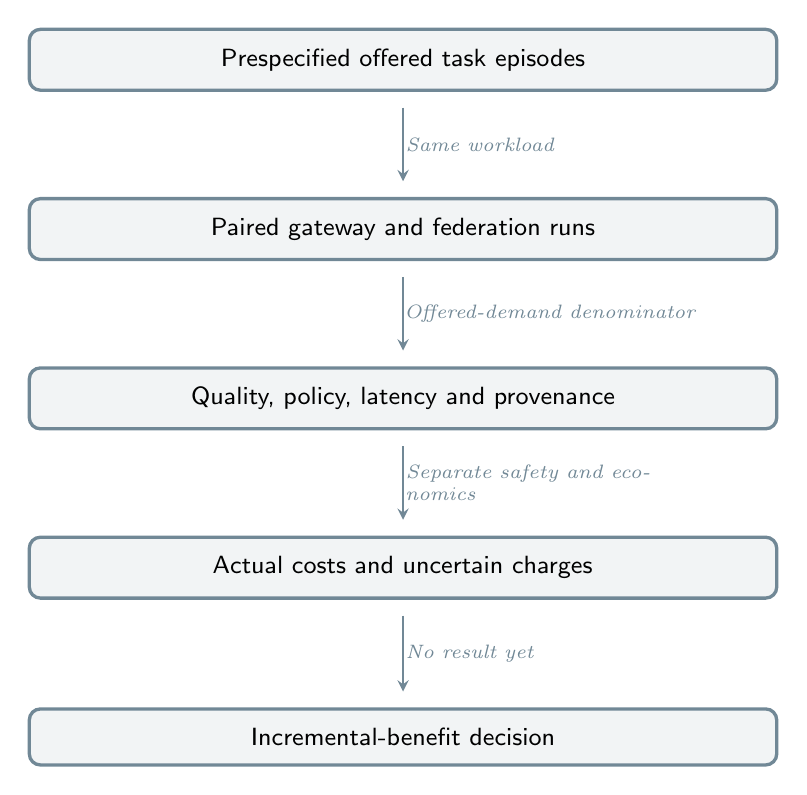
\begin{tikzpicture}[x=1cm,y=1cm,>=stealth,story node/.style={draw=blue!65,very thick,rounded corners=4pt,align=center,text width=9cm,font=\small\sffamily,fill=blue!6,inner sep=7pt}]
\node[story node] (tasks) at (0,0.00) {Prespecified offered task episodes};
\node[story node] (pair) at (0,-2.15) {Paired gateway and federation runs};
\node[story node] (outcomes) at (0,-4.30) {Quality, policy, latency and provenance};
\node[story node] (cost) at (0,-6.45) {Actual costs and uncertain charges};
\node[story node] (decision) at (0,-8.60) {Incremental-benefit decision};
\draw[->,thick,blue!65,shorten <=2mm,shorten >=2mm] (tasks) -- node[midway,right,font=\scriptsize\itshape,align=left,text width=3.8cm,fill=white,inner sep=1pt] {Same workload} (pair);
\draw[->,thick,blue!65,shorten <=2mm,shorten >=2mm] (pair) -- node[midway,right,font=\scriptsize\itshape,align=left,text width=3.8cm,fill=white,inner sep=1pt] {Offered-demand denominator} (outcomes);
\draw[->,thick,blue!65,shorten <=2mm,shorten >=2mm] (outcomes) -- node[midway,right,font=\scriptsize\itshape,align=left,text width=3.8cm,fill=white,inner sep=1pt] {Separate safety and economics} (cost);
\draw[->,thick,blue!65,shorten <=2mm,shorten >=2mm] (cost) -- node[midway,right,font=\scriptsize\itshape,align=left,text width=3.8cm,fill=white,inner sep=1pt] {No result yet} (decision);
\end{tikzpicture}
\caption{The proposed 90-day comparison asks whether federation adds useful, policy-permitted service beyond a gateway that already permits separately approved external access. Paired task quality, safety, and actual cost must be evaluated separately; no pilot result is available.}
\par\smallskip{\scriptsize Source-linked claims: C18, C19, C23; evidence links appear in the claim notes.}
\end{figure}
\section{Limitations}
\begin{itemize}
\item The starting documentation and PEARC\textquoteright{}26 paper were not inspected. The reported 2026-10-31 review date is historical project information, not an access date established here.
\item The evidence is a bounded selection with truncated extracts and pointer-only originals; it does not support an exhaustive semantic review.
\item The conditional enforcement and accounting arguments are not implementation proofs, independent verification, or deployment evidence.
\item Prices, contractual charging bounds, campus policies, cost ledgers, workload traces, benchmark results, and recipient compliance remain unestablished.
\item Saved research session 36e06a52-e138-48ee-9ccf-1519bb6faedc ended with an incomplete review; call 18 (skeptic) was not successfully completed. Earlier findings remain available, but this process limitation prevents claiming that the planned adversarial review was fully performed.
\item Saved research session d82391f1-956a-4546-adfd-20f030e33688 ended with an incomplete review; call 12 (skeptic) was not successfully completed. Earlier findings remain available, but this process limitation prevents claiming that the planned adversarial review was fully performed.
\end{itemize}
\section{Open obligations}
\begin{itemize}
\item Retrieve and archive \url{https://mindrouter.ai/documentation.html} and \url{https://ai4ra.uidaho.edu/wp-content/uploads/2026/04/Sheneman_MindRouter_PEARC26_Short_Paper.pdf} with actual access dates and versions; verify feature descriptions and changed claims.
\item Obtain security, data-owner, legal, and procurement decisions on classification inheritance, approved destinations, retention, contracts, audit, revocation semantics, and in-flight handling.
\item Implement and independently inspect complete mediation, immutable request binding, serialized release, exclusive ownership and fencing, replay controls, durable nested reservations, and recovery.
\item Obtain dated API rates and enforceable liability bounds; replace hypothetical costs with campus evidence and reconcile cash flow, depreciation, replacement, and staff scope.
\item Approve task rubrics, deadlines, provenance requirements, evaluators, sampling units, fairness references, administrative ceilings, and stop/go authority.
\item Execute adversarial tests and an affordable, adequately sampled 90-day pilot; assess federation's incremental benefit rather than assuming it.
\end{itemize}
\section{Conclusions}
The saved evidence supports conditional architectural constraints, not a finding that university federation delivers reliable, economical AI access.

Hard-budget safety requires enforceable charge bounds and retained uncertain holds; authorization safety requires a precisely defined, completely mediated release boundary.

Federation should advance only if an approved comparison demonstrates material policy-permitted benefit over a campus gateway with separately approved external access. Otherwise the smaller trust boundary remains the provisional alternative, not an empirically established winner.

\appendix
\section{Claim and source notes}
These notes identify the saved evidence for claims used in the article. The complete claim register and reasoning are retained in the paper record.
\begin{sloppypar}
\small
\begin{description}
\item[C21] Substituting upper liability bounds for both services' actual costs can falsely favor federation because baseline cost enters the economic contrast with a negative coefficient. The saved counterexample has equal actual costs and universal success, yet unequal unresolved upper bounds produce an apparently favorable federation contrast. \textit{Status: }established.
\textit{Evidence: }[Research session 2, artifact 4]
\item[C22] A proposed repair propagates charge intervals directionally: an upper economic contrast uses federation upper costs and baseline lower costs, while a lower contrast uses federation lower costs and baseline upper costs. \textit{Status: }conjecture.
\textit{Evidence: }[Research session 2, artifact 4]
\item[C23] A proposed 90-day pilot must separate safety-stop, statistical no-go, and inconclusive outcomes and must establish federation's incremental benefit over the gateway baseline before supporting deployment. Its operational protocol, evaluator approvals, administrative ceilings, and final stop/go criteria remain incomplete. \textit{Status: }unresolved.
\textit{Evidence: }[Research session 1, artifact 1], [Research session 1, artifact 6], [Research session 2, artifact 4], [Research session 1]
\item[C16] WDRR scheduling weights alone do not establish starvation freedom or bounded latency when requests face heterogeneous model fit, unavailable compatible capacity, blocking, or cold starts. \textit{Status: }limitation.
\textit{Evidence: }[Research session 1, artifact 3], [Research session 1, artifact 6]
\item[C17] No observed comparison establishes task quality, provenance reproducibility, latency, throughput, availability, compatible GPU capacity, fairness, administrative burden, or net federation benefit across the four alternatives. \textit{Status: }unresolved.
\textit{Evidence: }[Research session 1], [Research session 1, artifact 5], [Research session 1, artifact 7]
\item[C18] The saved confirmatory pilot design compares federation with the gateway baseline using paired task episodes sampled before admission. Under its stated independence and bounded-cost assumptions, it proposes fixed-sample bounds and multiplicity control for a 5\% false statistical go probability. \textit{Status: }conjecture.
\textit{Evidence: }[Research session 2, artifact 4], [Research session 1, artifact 6]
\item[C19] The saved design reports approximately 2,820 independent task pairs for completion precision of plus or minus 3 percentage points and 4,061 pairs for federation-advantage precision of plus or minus 5 points; these are planning calculations, not achieved sample sizes or power results. \textit{Status: }conjecture.
\textit{Evidence: }[Research session 2, artifact 4], [Research session 1, artifact 6]
\item[C20] The earlier exploratory target of 30 tasks per stratum and a point estimate of at least 10 percentage points with an interval excluding zero was superseded by a stronger confidence-bound gate; the earlier rule does not establish a true advantage exceeding 10 points. \textit{Status: }established.
\textit{Evidence: }[Research session 1, artifact 6]
\item[C11] Releasing a reservation solely because a call timed out or was cancelled can violate a hard budget when the original call may still be charged. The saved example permits two liabilities of 6 against a cap of 10 if an uncertain first hold is released before retry. \textit{Status: }established.
\textit{Evidence: }[Research session 1, artifact 7], [Research session 2, artifact 2]
\item[C12] Within the reservation model, a zero budget with no prior funding cannot admit a new positive-liability call; budget exhaustion must therefore produce denial or an independently authorized non-paid alternative, not paid retry escalation. \textit{Status: }established.
\textit{Evidence: }[Research session 2, artifact 2], [Project overview]
\item[C13] A defensible cost comparison requires a common workload and horizon, separate sunk, incremental, and fully loaded accounting, and costs per active researcher and useful completed episode. Current API prices, campus ledgers, contractual liabilities, and federation overhead are not established. \textit{Status: }unresolved.
\textit{Evidence: }[Project overview], [Strategy 2: Ownership cost and task quality], [Research session 1, artifact 2], [Research session 1, artifact 8]
\item[C14] The saved hypothetical cohort contains 2,000 monthly root tasks, including 200 sensitive campus-only tasks, with local admission of 1,000 tasks. Under assumed average joint usefulness of $0.80$ for each local stratum, those admissions imply 800 expected useful local completions, including 160 sensitive completions; these are expectations, not observations or service guarantees. \textit{Status: }established.
\textit{Evidence: }[Research session 1, artifact 8], [Research session 1]
\item[C15] The available evidence does not establish a numerical break-even point or economic superiority for federation over the gateway baseline. Any comparison must hold workload, cost basis, quality, latency, and acceptance rules fixed and must account for genuinely usable, policy-permitted peer capacity. \textit{Status: }unresolved.
\textit{Evidence: }[Research session 1, artifact 2], [Research session 1, artifact 8], [Research session 1, artifact 1]
\item[C10] A conditional accounting argument preserves every account's hard cap if all billable actions have enforceable upper liability bounds, admission reserves atomically across applicable limits, unresolved liabilities retain their holds, and settlement never exceeds its reservation. \textit{Status: }conjecture.
\textit{Evidence: }[Research session 2, artifact 2], [Research session 1, artifact 3]
\end{description}
\end{sloppypar}
\section{Editorial writing sources}
These sources informed manuscript organization and writing methods, not the scientific evidence or findings.
\begin{itemize}
\item PLOS ONE \textemdash{} Manuscript and Reporting Guidelines (general): \url{https://journals.plos.org/plosone/s/submission-guidelines}
\item EASE \textemdash{} Guidelines for Authors of Scientific Articles (full text) (general): \url{https://pmc.ncbi.nlm.nih.gov/articles/PMC4130677/}
\end{itemize}
\end{document}
